% Author: Izaak Neutelings (December 2020)
\documentclass[border=3pt,tikz]{standalone}
\usepackage{amsmath}
\usepackage{tikz}
\usepackage{physics}
\usetikzlibrary{calc}
\tikzset{>=latex} % for LaTeX arrow head
\usepackage{xcolor}
\colorlet{veccol}{green!45!black}
\colorlet{myred}{red!90!black}
\colorlet{myblue}{blue!90!black}
\colorlet{myorange}{orange!90!black}
\colorlet{mygreen}{green!60!black}
%\colorlet{mypurple}{blue!50!red!80!black!80}
%\tikzstyle{vector}=[->,very thick,veccol]
%\usetikzlibrary{arrows.meta}

\begin{document}


% LOCAL MINIMUM
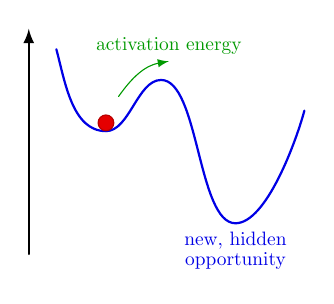
\begin{tikzpicture}[line cap=round,every node/.style={scale=0.7}] %[xscale=4,yscale=2]
  \def\xmax{3.5}
  \def\ymax{2.6}
  %\draw[->,thick] (-0.1*\ymax,0) -- (\xmax,0) node[below left=-2] {Time};
  \draw[->,thick] (0,-0.1*\ymax) -- (0,\ymax); % node[above left,rotate=90] {Opportunity};
  \draw[thick,myblue]
    (0.10*\xmax,0.90*\ymax) to[out=-75,in=180,looseness=0.9]
    (0.28*\xmax,0.5*\ymax) coordinate (A) to[out=0,in=180,looseness=0.8]
    (0.48*\xmax,0.75*\ymax) to[out=0,in=180,looseness=0.6]
    (0.75*\xmax,0.05*\ymax) node[below=1,align=center] {new, hidden\\[-2] opportunity} to[out=0,in=-105,looseness=0.6]
    (\xmax,0.6*\ymax);
  \draw[myred!80!black,fill=myred] ([yshift=3]A) circle(0.1);
  \draw[->,mygreen]
    (A)++(70:0.18*\ymax) to[out=55,in=-170]++ (35:0.3*\ymax)
    node[above] {activation energy};
\end{tikzpicture}


\end{document}